\chapter{Conclusion}
\section{Overview}
% General overview of techniques

\section{Skill Development}
This project helped me develop skills relating to graphics and coordinate
geometry a lot more, before partaking in the project I was not confident in my
skills doing any programming that drew to the screen. I also gained a good
understanding of novel methods for visualising multi-variate data and a better
understanding of the field of data visualisation which I think is important to
explore further especially with uses in AI and Machine Learning where
multi-variate data is common.

\section{Personal Reflection}
% Hard to funnel this into a goal
The nature of this project was such that

\section{Future Development}
One concept for an extension of this I enjoy but wasn't possible to complete due
to budgetary constraints and access to materials would be to control the program
using a dance pad for rhythm games. Perhaps at an event like Leeds Light Night a
large projection of the image could be made and a people invited to step onto a
dance pad to control the artwork.

\begin{figure}[H]
    \centering
    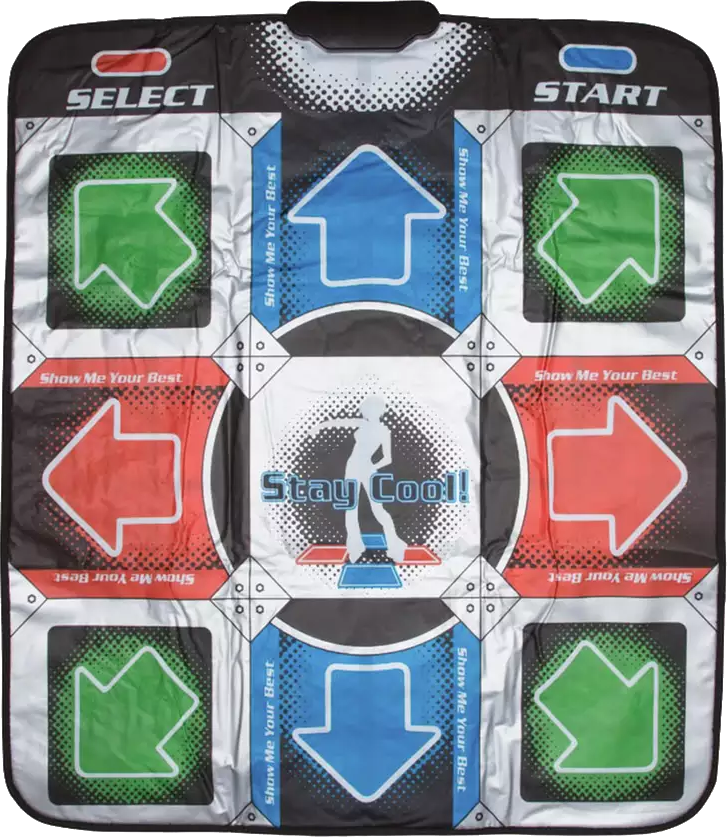
\includegraphics[width=0.3\textwidth]{dancepad}
    \caption{An eight-direction dance pad would map to most of the controls in
    this program}
\end{figure}

A few other options I considered were having a 3D models represent the image.
Similar to the giant's causeway, these would be extrusions of polygons through
space. Also a full map overview where the user could choose two points on the
history tree and view, in 2D or 3D a `map' of what they saw in that time frame.

Outside of the space of the art itself, I would like to develop the technique in
\autoref{sonicnav} further to see if it would work for other users and perhaps
extend it to encode more information, this would require more in depth study.

\section{Ethical and Legal Considerations}
This project does not handle any personal data, nor deals with identification of
people from data. There is no subject matter that may offend or otherwise effect
groups of people. 

However there is a question over ownership and who owns images produced by this
program if they are indistinguishable from Viner's own work.  One point to
consider is that where his work is pen-plotter images on listing paper, this is
purely computer generated imagery. 

Of course, also the provenance associated with the work is also completely
different; in the case of Prado's Mona List for example, it's clear that despite
being made around the same time, in the same workshop, and of the same subject
it is a separate piece of work with a different story. This perhaps is not the
best example however the creator of the Prado version likely worked in da
Vinci's studio at the time \citep{museodelprado_MonaLisa}. 

It's also worth mentioning the fair dealing exception to UK copyright law which
says that you are allowed to ``copy limited extracts of work for non-commercial
research or private study"\citep{govuk_copyright}. However I am unsure if this
legal protection extends to \emph{the potential for generating} copies of work.
It is clear to me however that I am not attempting to reproduce directly and
instead explore the techniques of creation of this work using completely
different technology.
